\documentclass[proceedings, preprint]{rmaa}

% The preprint option sets the first page header to contain the name
% of the conference. It will be ignored when typesetting the final
% volume. 

%%%
%%% Load any optional packages you need here with \usepackage
%%% 

% This allows compact, in-paragraph, and as-paragraph  versions of the
% standard itemize and enumerate environments. 
\usepackage{paralist}

% These are used in one of the graphics examples
\usepackage{psfrag,color}
\usepackage{comment}
\includecomment{comment} 
%%%
%%% Define any personal macros here
%%% 

% These are some I use in typesetting example code
\newcommand{\bs}{\textbackslash}
\newcommand{\CS}[1]{\texttt{\textbackslash #1}}
\newenvironment{Example}
{\begin{list}{}{\setlength{\leftmargin}{5pt}\setlength{\rightmargin}{5pt}}\item[]}
  {\end{list}}

  
%%%
%%% Article preamble commands (title, authors, abstract, etc.) 
%%% None of these produce any output themselves, they just set things 
%%% up for \maketitle
%%%

% This is only used for making the header for the preprint version
\SetYear{2014}
\SetConfTitle{Galaxy Evolution: Theory and Observations}

% Please use mixed case here, since this title gets propagated onto
% the web page, ADS entry, etc. 
\title{GAIA's view on the metallicities of the milky way} 

% For the conference proceedings, the author affiliations should be
% subscripted, using \altaffil and/or \altaffilmark + \altaffiltext
% Note that \altaffilmark goes after a comma and that `and' is spelt
% out.
\author{
  Fernandez-trincado, J.G,\altaffilmark{1} 
  Figueras, F, \altaffilmark{2}  
  Garavito-Camargo, J.N,\altaffilmark{3}
  Kawata, Daisuke. \altaffilmark{4}
  Marin, P,\altaffilmark{5}
  Munoz, J.T, \altaffilmark{6}}

% Note that \altaffil, \altaffilmark go inside the scope of the
% \author{...} command but \altaffiltext is outside it. 
\altaffiltext{1}{...}

\altaffiltext{2}{...}

\altaffiltext{3}{...}
\altaffiltext{4}{...}
\altaffiltext{5}{...}
\altaffiltext{6}{...}
% Authors for running headers - surnames only, et al. if more than 3. 
\shortauthor{Fernandez-Trincado et al}
% Title for running header
\shorttitle{RevMexAA(SC) Demo Document}

% List of authors used to construct table of contents
\listofauthors{Fernandez-Trincado et al}
% Each author in Surname, Initials format, used in generating Author
% Index entries.
\indexauthor{Henney, W. J.}
\indexauthor{Collaborator, A.}
\indexauthor{Author, L.}

% English abstract
\abstract{}

% Spanish abstract - leave blank and it will be translated by the
% editors. 
%\resumen{Presentamos los resultados de observaciones a frecuencias
%  m\'ultiples del proplyd LV~2 (M42~167--317) en la nebulosa de Ori\'on,
%  concentrando sobre nuestra analis\'\i{}s del ``microjet'' unidireccional
%  que sale del frente de ionizci\'on del proplyd.}


% Keywords must be from the standard list and in alphabetical order. 
% You should have no more than SIX different keywords. 
\addkeyword{GAIA}
\addkeyword{}
\addkeyword{}
\addkeyword{}

%%%
%%% Beginning of document proper
%%%
\begin{document}
% Typeset article header
\maketitle


\section{Introduction}

\section{Test particle simulation}

\section{SPH simulation}

We also use the SPH simulation made by (Daisuke ref) in which a MW galaxy.

\subsection{simulation parameters}

This simulation have 10000 Particles...
Initial conditions etc...
Extinction model

\section{Results}

We assume that all stars in the simulation are Red Clump stars with $M_{v} = 1.274$.
GAIA's field of view would be constrained to $v < 16.5$ (check this it could be larger), this 
field is illustrated in Fig.~\ref{•}

\begin{figure}
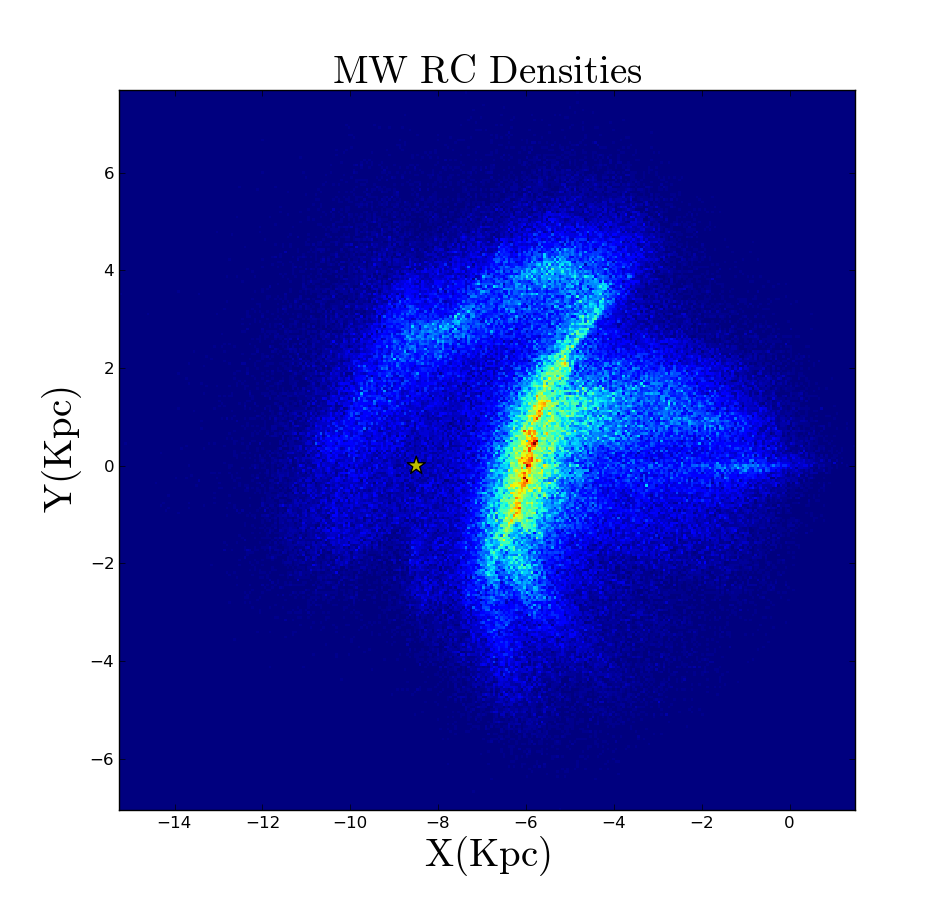
\includegraphics[scale=0.3]{GalaxyRC.png}
{\label{GAIA field of view}}
\end{figure}

\begin{figure}
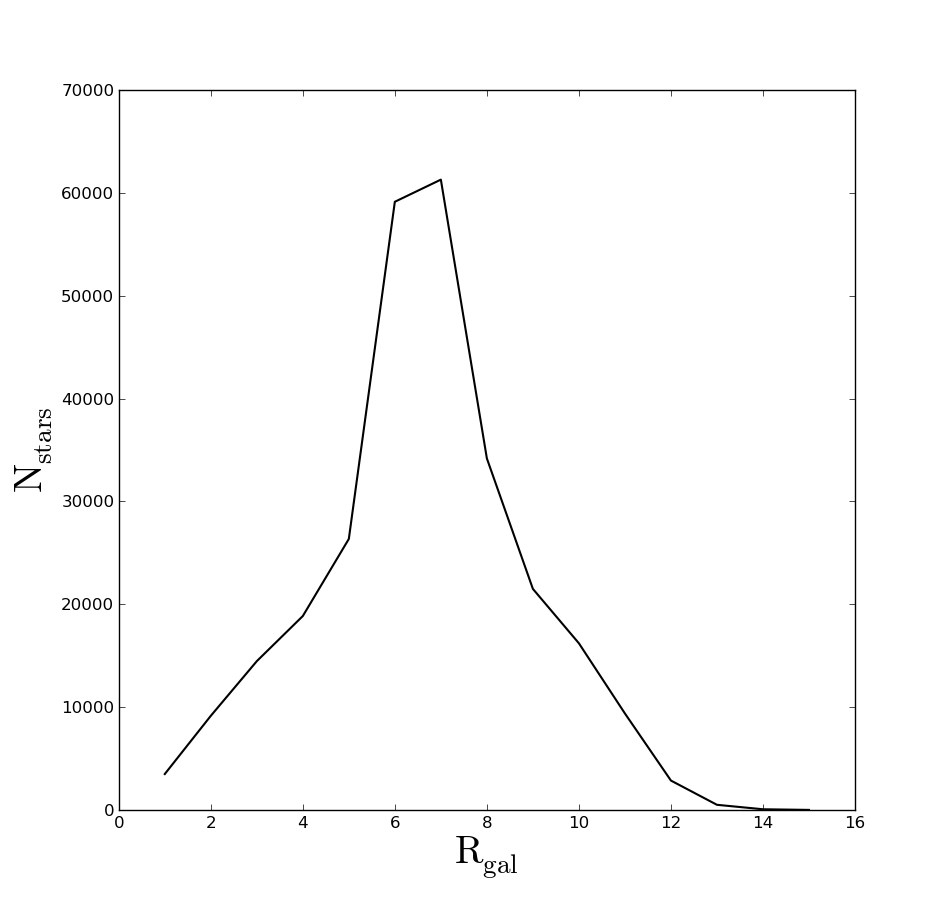
\includegraphics[scale=0.3]{histRealandobs.png}
\end{figure}

\begin{figure}
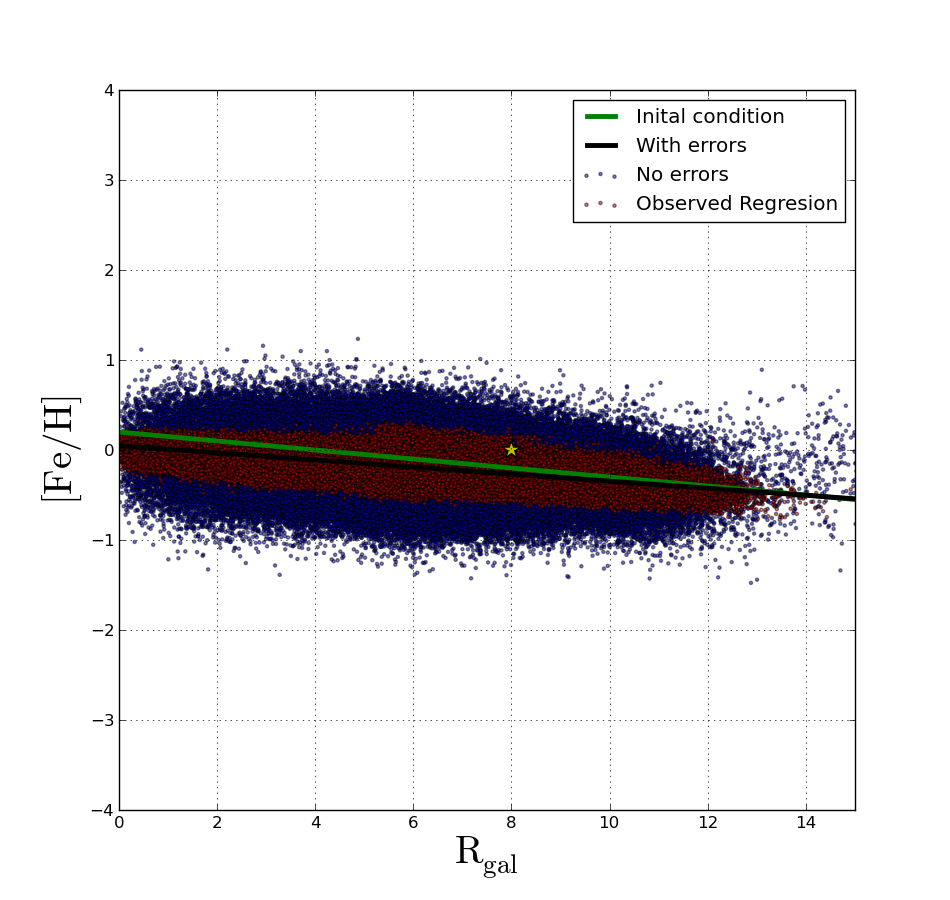
\includegraphics[scale=0.3]{ObsZandreal.png}
\end{figure} 

\subsection{SPH simulation}



\section{Discussion}

\section{Conclusions}

\begin{thebibliography}
\bibitem[Arthur \& Hoare(2006)]{2005astro.ph.11035A} Arthur, S.~J., \&
Hoare, M.~G.\ 2006, \apj, in press (astro-ph/0511035)

\end{thebibliography}


\end{document}
